% Options for packages loaded elsewhere
\PassOptionsToPackage{unicode}{hyperref}
\PassOptionsToPackage{hyphens}{url}
\PassOptionsToPackage{dvipsnames,svgnames,x11names}{xcolor}
%
\documentclass[
  xelatex,
  ja=standard]{bxjsarticle}

\usepackage{amsmath,amssymb}
\usepackage{iftex}
\ifPDFTeX
  \usepackage[T1]{fontenc}
  \usepackage[utf8]{inputenc}
  \usepackage{textcomp} % provide euro and other symbols
\else % if luatex or xetex
  \usepackage{unicode-math}
  \defaultfontfeatures{Scale=MatchLowercase}
  \defaultfontfeatures[\rmfamily]{Ligatures=TeX,Scale=1}
\fi
\usepackage{lmodern}
\ifPDFTeX\else  
    % xetex/luatex font selection
  \setmainfont[BoldFont=Noto Sans CJK JP]{Noto Serif CJK JP}
\fi
% Use upquote if available, for straight quotes in verbatim environments
\IfFileExists{upquote.sty}{\usepackage{upquote}}{}
\IfFileExists{microtype.sty}{% use microtype if available
  \usepackage[]{microtype}
  \UseMicrotypeSet[protrusion]{basicmath} % disable protrusion for tt fonts
}{}
\makeatletter
\@ifundefined{KOMAClassName}{% if non-KOMA class
  \IfFileExists{parskip.sty}{%
    \usepackage{parskip}
  }{% else
    \setlength{\parindent}{0pt}
    \setlength{\parskip}{6pt plus 2pt minus 1pt}}
}{% if KOMA class
  \KOMAoptions{parskip=half}}
\makeatother
\usepackage{xcolor}
\setlength{\emergencystretch}{3em} % prevent overfull lines
\setcounter{secnumdepth}{5}
% Make \paragraph and \subparagraph free-standing
\ifx\paragraph\undefined\else
  \let\oldparagraph\paragraph
  \renewcommand{\paragraph}[1]{\oldparagraph{#1}\mbox{}}
\fi
\ifx\subparagraph\undefined\else
  \let\oldsubparagraph\subparagraph
  \renewcommand{\subparagraph}[1]{\oldsubparagraph{#1}\mbox{}}
\fi


\providecommand{\tightlist}{%
  \setlength{\itemsep}{0pt}\setlength{\parskip}{0pt}}\usepackage{longtable,booktabs,array}
\usepackage{calc} % for calculating minipage widths
% Correct order of tables after \paragraph or \subparagraph
\usepackage{etoolbox}
\makeatletter
\patchcmd\longtable{\par}{\if@noskipsec\mbox{}\fi\par}{}{}
\makeatother
% Allow footnotes in longtable head/foot
\IfFileExists{footnotehyper.sty}{\usepackage{footnotehyper}}{\usepackage{footnote}}
\makesavenoteenv{longtable}
\usepackage{graphicx}
\makeatletter
\def\maxwidth{\ifdim\Gin@nat@width>\linewidth\linewidth\else\Gin@nat@width\fi}
\def\maxheight{\ifdim\Gin@nat@height>\textheight\textheight\else\Gin@nat@height\fi}
\makeatother
% Scale images if necessary, so that they will not overflow the page
% margins by default, and it is still possible to overwrite the defaults
% using explicit options in \includegraphics[width, height, ...]{}
\setkeys{Gin}{width=\maxwidth,height=\maxheight,keepaspectratio}
% Set default figure placement to htbp
\makeatletter
\def\fps@figure{htbp}
\makeatother

\renewcommand{\thefootnote}{\arabic{footnote}}
\makeatletter
\@ifpackageloaded{tcolorbox}{}{\usepackage[skins,breakable]{tcolorbox}}
\@ifpackageloaded{fontawesome5}{}{\usepackage{fontawesome5}}
\definecolor{quarto-callout-color}{HTML}{909090}
\definecolor{quarto-callout-note-color}{HTML}{0758E5}
\definecolor{quarto-callout-important-color}{HTML}{CC1914}
\definecolor{quarto-callout-warning-color}{HTML}{EB9113}
\definecolor{quarto-callout-tip-color}{HTML}{00A047}
\definecolor{quarto-callout-caution-color}{HTML}{FC5300}
\definecolor{quarto-callout-color-frame}{HTML}{acacac}
\definecolor{quarto-callout-note-color-frame}{HTML}{4582ec}
\definecolor{quarto-callout-important-color-frame}{HTML}{d9534f}
\definecolor{quarto-callout-warning-color-frame}{HTML}{f0ad4e}
\definecolor{quarto-callout-tip-color-frame}{HTML}{02b875}
\definecolor{quarto-callout-caution-color-frame}{HTML}{fd7e14}
\makeatother
\makeatletter
\makeatother
\makeatletter
\makeatother
\makeatletter
\@ifpackageloaded{caption}{}{\usepackage{caption}}
\AtBeginDocument{%
\ifdefined\contentsname
  \renewcommand*\contentsname{目次}
\else
  \newcommand\contentsname{目次}
\fi
\ifdefined\listfigurename
  \renewcommand*\listfigurename{図一覧}
\else
  \newcommand\listfigurename{図一覧}
\fi
\ifdefined\listtablename
  \renewcommand*\listtablename{表一覧}
\else
  \newcommand\listtablename{表一覧}
\fi
\ifdefined\figurename
  \renewcommand*\figurename{図}
\else
  \newcommand\figurename{図}
\fi
\ifdefined\tablename
  \renewcommand*\tablename{表}
\else
  \newcommand\tablename{表}
\fi
}
\@ifpackageloaded{float}{}{\usepackage{float}}
\floatstyle{ruled}
\@ifundefined{c@chapter}{\newfloat{codelisting}{h}{lop}}{\newfloat{codelisting}{h}{lop}[chapter]}
\floatname{codelisting}{コード}
\newcommand*\listoflistings{\listof{codelisting}{コード一覧}}
\makeatother
\makeatletter
\@ifpackageloaded{caption}{}{\usepackage{caption}}
\@ifpackageloaded{subcaption}{}{\usepackage{subcaption}}
\makeatother
\makeatletter
\@ifpackageloaded{tcolorbox}{}{\usepackage[skins,breakable]{tcolorbox}}
\makeatother
\makeatletter
\@ifundefined{shadecolor}{\definecolor{shadecolor}{rgb}{.97, .97, .97}}
\makeatother
\makeatletter
\makeatother
\makeatletter
\makeatother
\ifLuaTeX
\usepackage[bidi=basic]{babel}
\else
\usepackage[bidi=default]{babel}
\fi
\babelprovide[main,import]{japanese}
% get rid of language-specific shorthands (see #6817):
\let\LanguageShortHands\languageshorthands
\def\languageshorthands#1{}
\ifLuaTeX
  \usepackage{selnolig}  % disable illegal ligatures
\fi
\usepackage[]{natbib}
\bibliographystyle{jecon}
\IfFileExists{bookmark.sty}{\usepackage{bookmark}}{\usepackage{hyperref}}
\IfFileExists{xurl.sty}{\usepackage{xurl}}{} % add URL line breaks if available
\urlstyle{same} % disable monospaced font for URLs
\hypersetup{
  pdftitle={民主的平和と商業的平和},
  pdfauthor={土井翔平},
  pdflang={ja},
  colorlinks=true,
  linkcolor={NavyBlue},
  filecolor={Maroon},
  citecolor={NavyBlue},
  urlcolor={NavyBlue},
  pdfcreator={LaTeX via pandoc}}

\title{民主的平和と商業的平和}
\usepackage{etoolbox}
\makeatletter
\providecommand{\subtitle}[1]{% add subtitle to \maketitle
  \apptocmd{\@title}{\par {\large #1 \par}}{}{}
}
\makeatother
\subtitle{国際公共政策学}
\author{土井翔平}
\date{2023-05-30}

\begin{document}
\maketitle
\ifdefined\Shaded\renewenvironment{Shaded}{\begin{tcolorbox}[interior hidden, frame hidden, sharp corners, borderline west={3pt}{0pt}{shadecolor}, boxrule=0pt, breakable, enhanced]}{\end{tcolorbox}}\fi

\hypertarget{ux6c11ux4e3bux7684ux5e73ux548c}{%
\section{民主的平和}\label{ux6c11ux4e3bux7684ux5e73ux548c}}

\textbf{民主的平和} (democratic peace: DP)
:「民主主義国\textbf{同士}は戦争をしない」という経験則

\begin{itemize}
\tightlist
\item
  1900年以降の二国間の政治体制の組み合わせとMID発生件数の関係
\item
  民主主義に関するデータセットについては \citet{kubo2016} や
  \citet{kasuya2014} を参考
\item
  \href{https://www.systemicpeace.org/polityproject.html}{Polity
  5}や\href{https://www.v-dem.net/}{V-Dem}
\end{itemize}

\begin{figure}[htpb]

{\centering 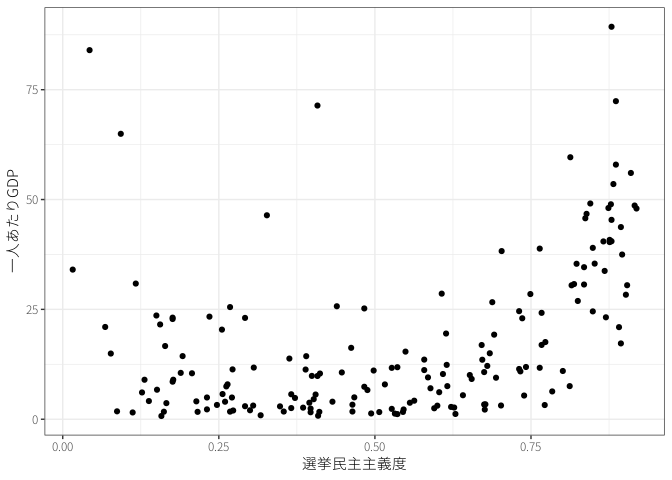
\includegraphics{democratic_peace_files/figure-pdf/unnamed-chunk-2-1.png}

}

\caption{政治体制の組み合わせと紛争頻度}

\end{figure}

\(\leadsto\)民主主義の測り方によって細部は異なるが、次のことが言える\citep{gleditsch1997}。

\begin{enumerate}
\def\labelenumi{\arabic{enumi}.}
\tightlist
\item
  民主主義国\textbf{同士}\(\leadsto\)軍事衝突ほぼなし
\item
  民主主義国は権威主義国\(\leadsto\)軍事衝突あり
\end{enumerate}

\(\leadsto\)国内政治や政治体制も考慮しなければ戦争と平和については分からない。

\begin{itemize}
\tightlist
\item
  これまでは国家をみんな同じ個人、一枚岩のアクターとして扱ってきた。
\end{itemize}

\hypertarget{ux653fux6cbbux4f53ux5236}{%
\subsection{政治体制}\label{ux653fux6cbbux4f53ux5236}}

政治体制の定義については様々

\(\leadsto\)民主主義と権威主義 (autocracy/authoritarian)
という二分法ではない。

\begin{itemize}
\tightlist
\item
  \textbf{競争的権威主義}、\textbf{選挙権威主義}:形式的には選挙を行っているが実質的には独裁\citep{gandhi2009}\footnote{東島雅晶「\href{https://chuokoron.jp/politics/118651.html}{恐怖支配から恩寵政治へ? 権威主義体制の変貌する統治手法}」(2022)
    中央公論;浅古泰史・東島雅昌「「\href{https://www.web-nippyo.jp/29067/}{民主主義
    vs.~権威主義」のゆくえ}」(2022) 経済セミナー10・11月号}
\item
  独裁のあり方にも様々(個人独裁、軍事政権、集団指導など)
\end{itemize}

長期的に見ると民主化かが進んでいる。

\begin{itemize}
\tightlist
\item
  近年は民主主義の後退 (\textbf{democracy backsliding})
  の懸念も主張されている。
\end{itemize}

\begin{figure}[htpb]

{\centering 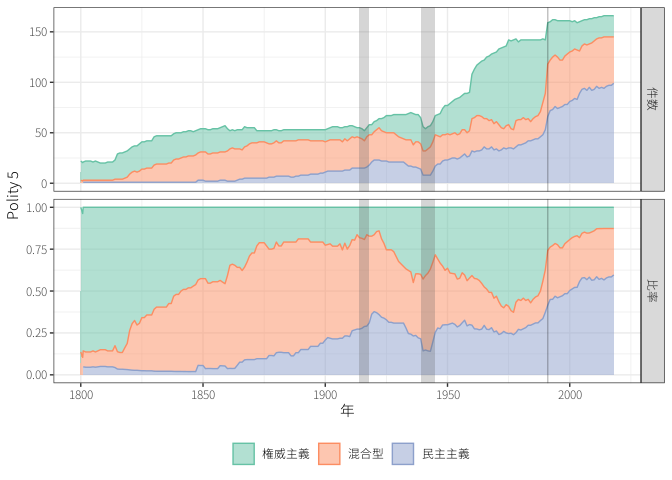
\includegraphics{democratic_peace_files/figure-pdf/unnamed-chunk-3-1.png}

}

\caption{政治体制の推移 (Polity V)}

\end{figure}

\begin{figure}[htpb]

{\centering 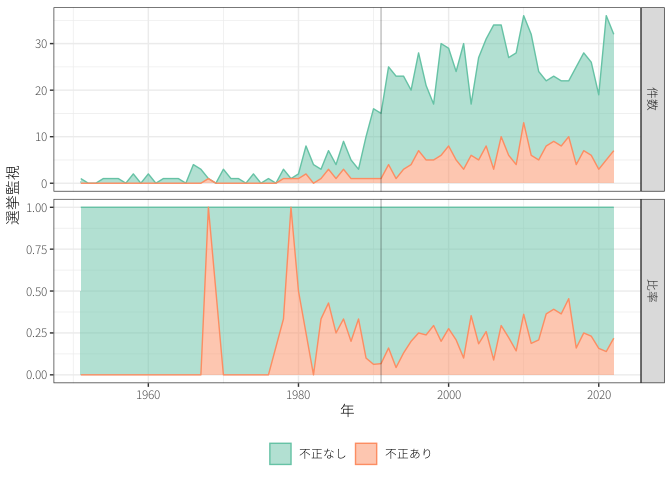
\includegraphics{democratic_peace_files/figure-pdf/unnamed-chunk-4-1.png}

}

\caption{政治体制の推移 (V-Dem)}

\end{figure}

政治体制は地域ごとに偏りがある。

\begin{figure}[htpb]

{\centering 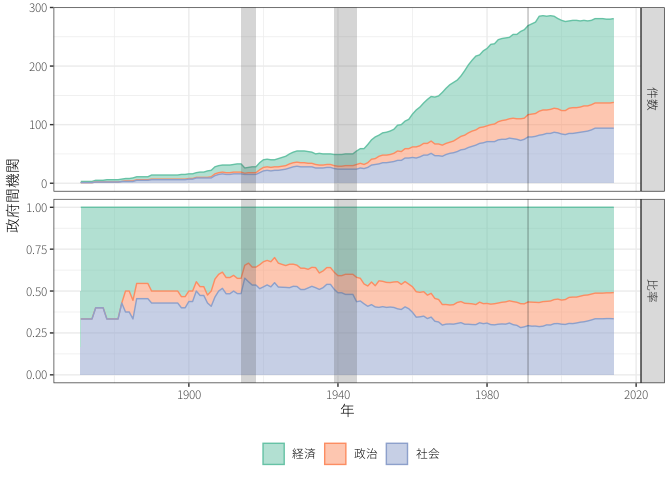
\includegraphics{democratic_peace_files/figure-pdf/unnamed-chunk-5-1.png}

}

\caption{政治体制の地理的分布}

\end{figure}

\hypertarget{ux6c11ux4e3bux7684ux5e73ux548cux306eux8ad6ux7406}{%
\subsection{民主的平和の論理}\label{ux6c11ux4e3bux7684ux5e73ux548cux306eux8ad6ux7406}}

民主主義\textbf{同士}では戦争をしないという謎を説明する論理が様々に提案されている。

\begin{itemize}
\tightlist
\item
  権威主義国による戦争についてはあまり触れないが、 \citet{weeks2012}
  や次の論考\footnote{安中進「\href{https://chuokoron.jp/international/122696.html}{独裁者はなぜ向こう見ずな戦争を起こすのか?――計量分析から考察する戦争}」(2023)
    中央公論}を参照
\end{itemize}

\hypertarget{ux30a2ux30abux30a6ux30f3ux30bfux30d3ux30eaux30c6ux30a3}{%
\subsubsection{アカウンタビリティ}\label{ux30a2ux30abux30a6ux30f3ux30bfux30d3ux30eaux30c6ux30a3}}

政治体制=国内政治のルール\(\leadsto\)政策に影響

\begin{itemize}
\tightlist
\item
  全ての国が同じように国力や富を追求するわけではない。
\item
  実際の政策決定過程は複雑な委任 (delegation)
  関係、\textbf{本人=代理人モデル} (principal-agent model)
\item
  有権者→政治家→官僚など
\end{itemize}

\begin{figure}[htpb]

{\centering 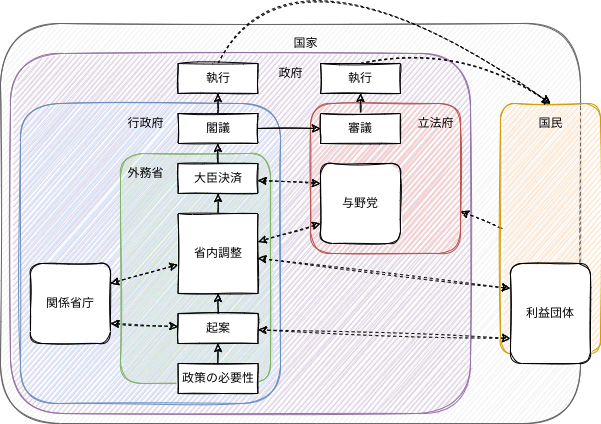
\includegraphics{figures/foreign_policy.drawio.png}

}

\caption{政策決定過程( \citet{yamakage2012} を参考に作成)}

\end{figure}

政治家は\textbf{選択民} (selectorate)
によって選出・排除される=アカウンタビリティ (accountability)

\begin{itemize}
\tightlist
\item
  アカウンタビリティ:結果に責任を負って、非難を受ける(究極的には役職からの追放)可能性があること\footnote{日本語では「説明責任」と呼ばれるが、説明をする(それだけでよい)責任ではない。}
\item
  選択民:政治的な指導者を(集団で)決定する権利を持つ人々
\end{itemize}

\(\leadsto\)政治的指導者は\textbf{勝利連合} (winning coalition)
を形成・維持することで\textbf{政治的生き残り} (political survival)
を図る\citetext{\citealp[第9章]{asako2018}; \citealp{buenodemesquita2013}}。

\begin{itemize}
\tightlist
\item
  主権国家体系では政治的指導者は国際社会や他国に対してアカウンタビリティを持っていない。
\end{itemize}

勝利連合の大きさは政治体制によって変わる。

\begin{itemize}
\tightlist
\item
  民主主義国:選択民は有権者全体であり、勝利連合は政権の獲得に必要な有権者の数
\item
  大統領制:勝利連合は選択民の約半分
\item
  議院内閣制で小選挙区制:選択民の1/4でも可能
\item
  権威主義国:選択民は一部のエリートや軍人であることが多く、勝利連合はそのうちの一部
\end{itemize}

\begin{figure}[htpb]

{\centering 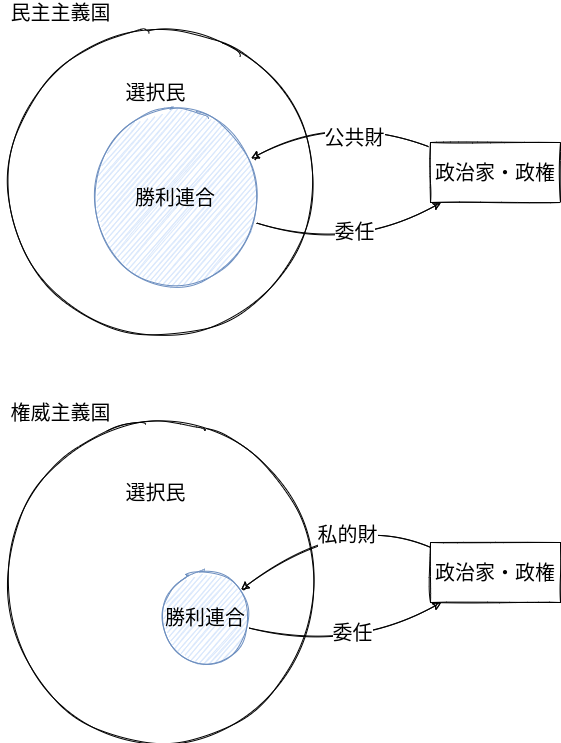
\includegraphics{figures/selectorate_theory.png}

}

\caption{政治体制、選挙民と勝利連合}

\end{figure}

政治家は有限の政策資源を配分して勝利連合を形成・維持

\(\leadsto\)選択民と勝利連合の大きさ\(\leadsto\)政策の違い\footnote{民主主義国の政治家が善人で、権威主義国の政治家が悪人であるとは限らない。}

\begin{itemize}
\tightlist
\item
  権威主義国:必要な勝利連合の規模が小さい\(\leadsto\)賄賂や利益誘導などの一部の個人に与えられる\textbf{私的財}
  (private goods)
\item
  民主主義国:必要な勝利連合の規模が大きい\(\leadsto\)経済成長や安全保障などの広く行き渡る\textbf{公共財}
  (public goods)
\item
  民主主義と権威主義のパフォーマンスに関しては次の論考\footnote{東島雅晶「\href{https://gendai.media/articles/-/91203}{民主主義と権威主義、どちらの「社会経済パフォーマンス」が上なのか?
    データ分析が示す驚きの結果}」(2022)
    現代ビジネス;安中進「\href{https://chuokoron.jp/politics/117870.html}{民主主義は権威主義に劣るのか?
    : コロナ禍における政治体制の実証分析}」(2021)
    中央公論;安中進「政治体制は豊かさや健康にどのような影響を及ぼすのか?」(2022)
    経済セミナー10・11月号}を参照
\end{itemize}

戦争において被害を受けるのは国民全体である/戦争を決定するのは一部の政治家

\(\leadsto\)民主主義国では多くの国民にアカウンタビリティを負っており、戦争では政治的に生き残りにくい。

\begin{itemize}
\tightlist
\item
  民主主義国が権威主義国とは戦うことは説明できない。
\item
  民主主義国の場合は選挙に負けるだけ/権威主義国の場合は革命やクーデタなどで政権の座を奪われ、処罰を受けることが多い\citep{goemans2008}
\end{itemize}

権威主義国は民主主義国の決意が低いと見積もって、強硬な姿勢になりやすい?

\begin{itemize}
\tightlist
\item
  権威主義国から攻撃することが多い\citep{reiter2003}
\end{itemize}

\hypertarget{ux900fux660eux6027}{%
\subsubsection{透明性}\label{ux900fux660eux6027}}

民主的平和の異なる説明として、情報の非対称性に着目するものがある。

\begin{itemize}
\tightlist
\item
  民主主義国では報道の自由\citep{van1997}や与野党の議論\citep{schultz1998}を通じて政治過程が比較的公開\(\leadsto\)情報の非対称(誤認される可能性)が減る
\end{itemize}

\begin{figure}[htpb]

{\centering 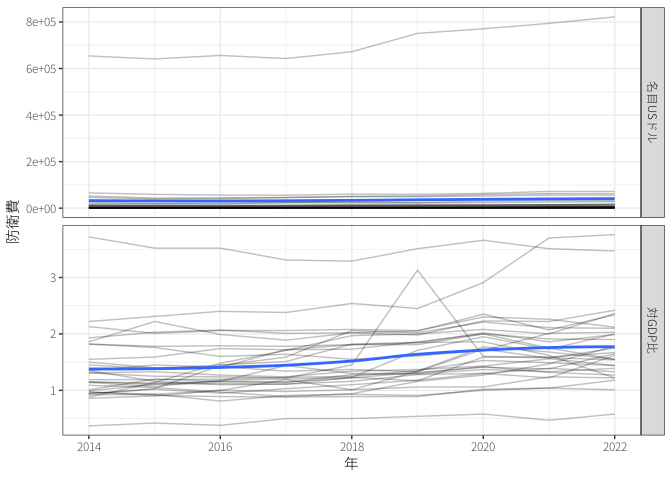
\includegraphics{democratic_peace_files/figure-pdf/unnamed-chunk-6-1.png}

}

\caption{表現の自由の地理的分布}

\end{figure}

\begin{itemize}
\tightlist
\item
  \textbf{観衆費用} (audience cost)
  \(\leadsto\)民主主義国の公開された威嚇には信憑性が高い\citep{fearon1994}。
\item
  観衆費用:言行不一致によって被る政治的コスト(例、国民からの支持の下落、選挙での敗北)
\end{itemize}

\begin{figure}[htpb]

{\centering \includegraphics[width=0.5\textwidth,height=\textheight]{democratic_peace_files/mediabag/GettyImages-11982326.jpg}

}

\caption{キューバ危機時のロバート・ケネディ米大統領}

\end{figure}

\begin{itemize}
\tightlist
\item
  (国内)観衆費用が存在するという研究\citep{tomz2007, kurizaki2015}
\item
  存在しない(大きな役割を果たしていない)という研究\citep[\citet{katagiri2019}]{snyder2011, trachtenberg2012}
\item
  権威主義国にも観衆費用は存在するという指摘\citep{weiss2013, weeks2008}
\item
  民主主義国の威嚇の信憑性は高くないという指摘\citep{downes2012}
\end{itemize}

透明性と民主的平和の関係に懐疑的な見方\citep{finel1999}

\begin{itemize}
\tightlist
\item
  民主主義の情報の政策生と権威主義国から攻撃することは整合的?
\end{itemize}

\hypertarget{ux898fux7bc4ux30a2ux30a4ux30c7ux30f3ux30c6ux30a3ux30c6ux30a3}{%
\subsubsection{規範・アイデンティティ}\label{ux898fux7bc4ux30a2ux30a4ux30c7ux30f3ux30c6ux30a3ux30c6ux30a3}}

民主主義国では対立を互いに平和的に解決するという規範が成立しており、それが国際関係にも波及?\citep{doyle1986, risse1995}

\begin{itemize}
\tightlist
\item
  民主主義国は一般的に平和的ではない。
\item
  民主主義国同士では互いに信頼しているので、暴力を用いない?
\item
  民主主義国同士:妥協により平和的に解決することが多い\citep{mousseau1998, dixon1994}
\item
  民主主義国の市民:民主主義を脅威とは捉えにくく、民主主義国同士の戦争に賛成しにくい\citep{tomz2013}
\item
  歴史的に見て民主主義国は権威主義国を必ず嫌うわけではない(例、冷戦期)
\end{itemize}

\hypertarget{ux5973ux6027ux653fux6cbbux5bb6}{%
\subsubsection{女性政治家}\label{ux5973ux6027ux653fux6cbbux5bb6}}

年々、女性参政権や女性議員の比率、女性の政治的指導は増加

\begin{figure}[htpb]

{\centering 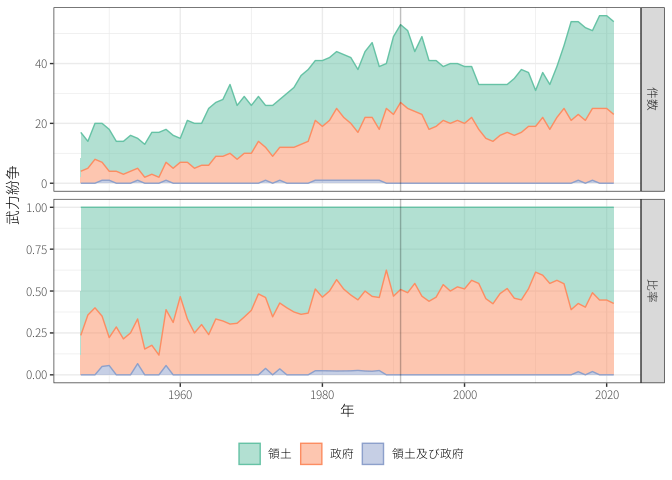
\includegraphics{democratic_peace_files/figure-pdf/unnamed-chunk-7-1.png}

}

\caption{女性参政権の推移}

\end{figure}

\begin{figure}[htpb]

{\centering 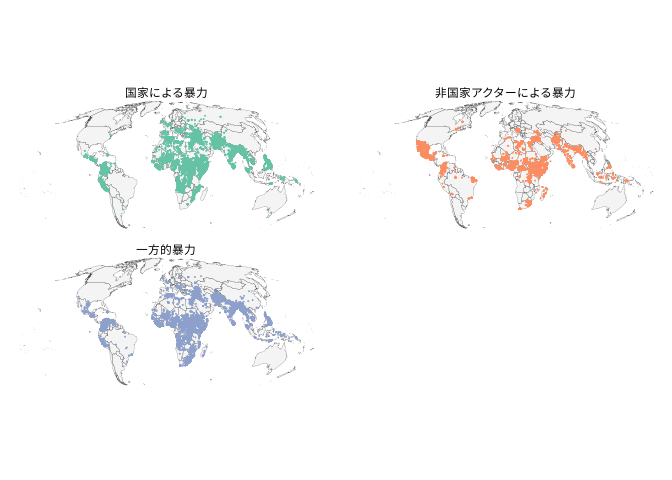
\includegraphics{democratic_peace_files/figure-pdf/unnamed-chunk-8-1.png}

}

\caption{女性議員比率の推移}

\end{figure}

\begin{figure}[htpb]

{\centering 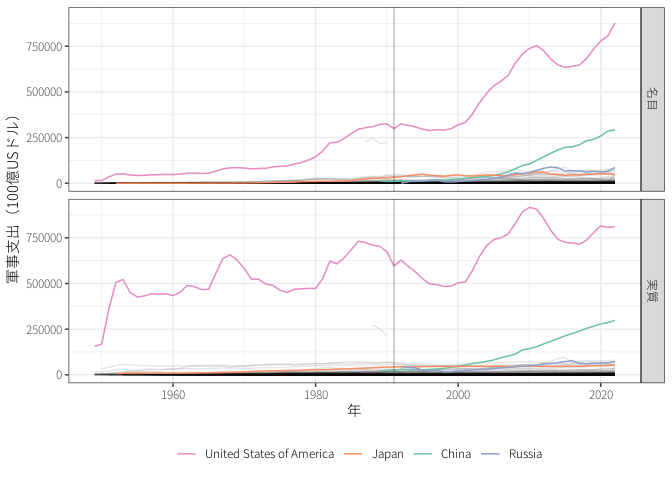
\includegraphics{democratic_peace_files/figure-pdf/unnamed-chunk-9-1.png}

}

\caption{女性の政治的指導者の推移}

\end{figure}

一般的に女性は男性に比べて武力行使に否定的で、平和的解決を望むと言われている

\(\leadsto\)女性の政治進出は平和をもたらす?

\begin{itemize}
\tightlist
\item
  ジェンダーの平等や女性議員の増加、女性参政権の拡大\(\leadsto\)民主主義国において武力行使や軍事費の減少\citep{reiter2015, barnhart2020}
\item
  平和的な社会で女性の政治進出が進んでいる?
\item
  女性の政治的指導者\(\leadsto\)対立的な行動を取りやすい\citep{koch2011, caprioli2001}
\item
  政治的指導者になるような女性は男性的である(ことが求められる)\citep{schramm2020}
\item
  女性の政治的指導者は他国から強硬な姿勢を取られやすい\citep{schwartz2020}
\end{itemize}

\hypertarget{ux6c11ux4e3bux4e3bux7fa9ux3068ux6c11ux610f}{%
\subsection{民主主義と民意}\label{ux6c11ux4e3bux4e3bux7fa9ux3068ux6c11ux610f}}

一般論として、民主主義のほうが権威主義に比べて広く市民の利益になる政策をしている。

\(\leadsto\)必ずしも民主主義(特に選挙)が民意を表しているとは言えない。

\begin{itemize}
\tightlist
\item
  社会的選択理論 (social choice
  theory):集団の意思決定(多数決)に関する研究\citep{sakai2015, sakai2016}
\end{itemize}

政策の好みと政党の好みは一致しないかもしれない。

\begin{tcolorbox}[enhanced jigsaw, colback=white, left=2mm, toptitle=1mm, title=\textcolor{quarto-callout-note-color}{\faInfo}\hspace{0.5em}{政策の好みと政党の好み}, toprule=.15mm, arc=.35mm, colbacktitle=quarto-callout-note-color!10!white, titlerule=0mm, opacityback=0, opacitybacktitle=0.6, bottomrule=.15mm, bottomtitle=1mm, rightrule=.15mm, coltitle=black, leftrule=.75mm, breakable, colframe=quarto-callout-note-color-frame]

5人の有権者がいて、A党とB党の3つの政策について、次のように好んでいる。

\end{tcolorbox}

\begin{longtable}[]{@{}ccccc@{}}
\caption{オストロゴルスキーのパラドックス\citep[p.23]{sakai2016}}\tabularnewline
\toprule\noalign{}
有権者 & 金融 & 外交 & 原発 & 支持政党 \\
\midrule\noalign{}
\endfirsthead
\toprule\noalign{}
有権者 & 金融 & 外交 & 原発 & 支持政党 \\
\midrule\noalign{}
\endhead
\bottomrule\noalign{}
\endlastfoot
1 & A & A & B & A \\
2 & A & B & A & A \\
3 & B & A & A & A \\
4 & B & B & B & B \\
5 & B & B & B & B \\
多数決の結果 & B & B & B & A \\
\end{longtable}

選び方によって結果は変わるかもしれない。

\begin{tcolorbox}[enhanced jigsaw, colback=white, left=2mm, toptitle=1mm, title=\textcolor{quarto-callout-note-color}{\faInfo}\hspace{0.5em}{選び方と政策}, toprule=.15mm, arc=.35mm, colbacktitle=quarto-callout-note-color!10!white, titlerule=0mm, opacityback=0, opacitybacktitle=0.6, bottomrule=.15mm, bottomtitle=1mm, rightrule=.15mm, coltitle=black, leftrule=.75mm, breakable, colframe=quarto-callout-note-color-frame]

9人の有権者がいて、4人の候補者(政策)について、次のように好んでいる。

\end{tcolorbox}

\begin{longtable}[]{@{}cccc@{}}
\caption{\citet{sakai2016}, p.43}\tabularnewline
\toprule\noalign{}
人数 & 4人 & 3人 & 2人 \\
\midrule\noalign{}
\endfirsthead
\toprule\noalign{}
人数 & 4人 & 3人 & 2人 \\
\midrule\noalign{}
\endhead
\bottomrule\noalign{}
\endlastfoot
1位 & A & C & D \\
2位 & B & B & B \\
3位 & C & A & C \\
4位 & D & D & A \\
\end{longtable}

\begin{itemize}
\tightlist
\item
  多数決

  \begin{itemize}
  \tightlist
  \item
    Aが最多の4人の支持を得る
  \end{itemize}
\item
  決選投票

  \begin{itemize}
  \tightlist
  \item
    1回目で2票しか得なかったDが落選
  \item
    決選投票ではCが5人の支持を得る\footnote{多数決の場合は票割れが起こってしまっている。}
  \end{itemize}
\item
  ボルダルール:1位に4点、2位に3点、3位に2点、4位に1点を与える

  \begin{itemize}
  \tightlist
  \item
    Aは24点、Bは27点、Cは24点、Dは15点
  \end{itemize}
\end{itemize}

\(\leadsto\)制度=ルールによって政策結果は変わりうる。

\begin{itemize}
\tightlist
\item
  選挙(多数決)の結果が民意を反映しているとは言えない。
\end{itemize}

\hypertarget{ux6c11ux4e3bux4e3bux7fa9ux306eux526fux4f5cux7528}{%
\subsection{民主主義の副作用}\label{ux6c11ux4e3bux4e3bux7fa9ux306eux526fux4f5cux7528}}

\hypertarget{ux65d7ux4e0bux7d50ux96c6ux52b9ux679c}{%
\subsubsection{旗下結集効果}\label{ux65d7ux4e0bux7d50ux96c6ux52b9ux679c}}

\textbf{旗下結集効果} (rally {[}'round the flag{]}
effect):戦争などの国家的危機において政府に対する支持率が急上昇する現象\citep{mueller1970}

\begin{figure}[htpb]

{\centering \includegraphics{democratic_peace_files/mediabag/1280px-George_W_Bush.png}

}

\caption{\href{https://commons.wikimedia.org/wiki/File:George_W_Bush_approval_ratings_with_events.svg}{ブッシュJr米大統領の支持率の推移}}

\end{figure}

\begin{itemize}
\tightlist
\item
  外敵の存在\(\leadsto\)集団の結束力が高まる。
\item
  野党が政府批判を控える。
\item
  ニュースが戦争に独占\(\leadsto\)政府に不都合な情報が流れにくい。
\item
  政府は国内問題を他国に転嫁する。
\end{itemize}

\(\leadsto\)情報を公開すれば誤認は減るが、世論に影響されやすくなる。

\hypertarget{ux967dux52d5ux6226ux4e89}{%
\subsubsection{陽動戦争}\label{ux967dux52d5ux6226ux4e89}}

政治家は陽動戦争 (\textbf{diversionary war}) を起こす誘因を持つ。

\begin{itemize}
\tightlist
\item
  政権基盤が不安定な政治家は旗下結集効果によって政治的生き残りが可能?
\item
  復活のためのギャンブル (gambling for resurrection) に賭ける?
\end{itemize}

陽動戦争理論が正しい\(\leadsto\)経済状況が悪い場合に戦争を起こしやすい?

\begin{itemize}
\tightlist
\item
  権威主義国はインフレ率が上がると敵対国と戦いやすい\citep{mitchell2004}
\item
  民主主義国では右派の政権はインフレ率や失業率が上昇すると紛争を起こしやすい\citep{arena2009, fordham1998}
\end{itemize}

陽動戦争理論が正しい\(\leadsto\)政治的に不安定な場合に戦争を起こしやすい?

\begin{itemize}
\tightlist
\item
  政治的生き残りが難しい場合には戦争を起こしにくく、国際危機の可能性は生き残りを困難にする\citep{chiozza2003}
\item
  民主主義国における政治的生き残りにとって重要な選挙の前ではなく、選挙後に戦争は起こりやすい\citep{gaubatz1991}
\end{itemize}

旗下結集効果を見込んだ陽動戦争(例、フォークランド紛争)はしばしば観察される/戦争の大部分を説明するわけではない。

\begin{itemize}
\tightlist
\item
  戦争のコストを埋め合わせるほど大きな旗下結集効果は珍しい?
\item
  戦争には政治家にとっても大きなコストとなりうる\citep{goemans2000}

  \begin{itemize}
  \tightlist
  \item
    選挙権威主義国で妥協あるいは敗北をすると政治的指導者は処罰されやすい
  \end{itemize}
\item
  大きなコストではないという見方も\citep{chiozza2004}
\end{itemize}

\hypertarget{ux5229ux76caux8a98ux5c0e}{%
\subsubsection{利益誘導}\label{ux5229ux76caux8a98ux5c0e}}

政策決定は、\textbf{官僚}(特に安全保障では軍部)や\textbf{利益団体}
(interest group) も影響する。

\begin{itemize}
\tightlist
\item
  官僚や軍人:国益だけでなく予算の拡大や昇進といった自己目的も追求

  \begin{itemize}
  \tightlist
  \item
    軍部の影響力の高い国は武力紛争を起こしやすい\citep{sechser2004, weeks2012}
  \item
    アメリカでは軍部が文民(背広組)よりも武力行使に慎重になりやすい。
  \end{itemize}
\item
  ロビー団体や大企業(軍産複合体など)が攻撃的な政策を取るように圧力をかける?

  \begin{itemize}
  \tightlist
  \item
    平和的な関係を求める企業によるロビー活動も起こる\(\leadsto\)必ずしも利益団体の存在が戦争を引き起こすとは言えない\citep{brooks2013}
  \item
    戦争から利益を得るものがいるため、そうしたアクターの圧力の結果であるという陰謀論に陥りやすい。
  \end{itemize}
\end{itemize}

\(\leadsto\)陽動戦争にせよ利益誘導にせよ、戦争のコストよりも大きな利益を政治家に提供できるのか?

\hypertarget{ux6c11ux4e3bux5316ux306bux3088ux308bux5e73ux548c}{%
\subsection{民主化による平和?}\label{ux6c11ux4e3bux5316ux306bux3088ux308bux5e73ux548c}}

民主主義国同士では戦争が起こらないという\textbf{相関}\(\neq\)民主主義国同士になれば平和が促進されるという\textbf{因果}

\begin{itemize}
\tightlist
\item
  自由市場経済の国は民主主義になりやすく、平和的関係を維持しやすい?\citep{gartzke2007}
\item
  友好国に囲まれている国や領土問題を解決した国が民主化している?\citep{thompson1996, gibler2010, gibler2014}\^{}
\item
  民主主義国はWW2においてはドイツ、冷戦においてはソビエト連邦という共通の脅威に直面していたので、友好関係を維持していた?\citep{farber1997, mcdonald2015}
\end{itemize}

仮に民主主義国同士と平和の間に因果関係\(\neq\)民主化が平和を促進

\begin{itemize}
\tightlist
\item
  新興民主主義国や民主化の過程にある国は戦争を起こしやすい\citep{mansfield1995}

  \begin{itemize}
  \tightlist
  \item
    国民が敵対的な感情を抱いている国が民主化\(\leadsto\)世論に影響されて攻撃的な政策?
  \end{itemize}
\end{itemize}

\hypertarget{ux5546ux696dux7684ux5e73ux548c}{%
\section{商業的平和}\label{ux5546ux696dux7684ux5e73ux548c}}

貿易のように国境を越えた経済活動の規模は年々拡大

\begin{itemize}
\tightlist
\item
  \textbf{経済的相互依存} (economic
  interdependence):国家が他国に経済的に依存し合っている状態
\end{itemize}

\hypertarget{ux5546ux696dux7684ux5e73ux548cux306eux8ad6ux7406}{%
\subsection{商業的平和の論理}\label{ux5546ux696dux7684ux5e73ux548cux306eux8ad6ux7406}}

\textbf{商業的平和論} (commercial peace
theory):経済的相互依存の規模が拡大\(\leadsto\)国家間での戦争は起こりにくい

\begin{itemize}
\tightlist
\item
  戦争によって経済的相互依存が低下\(\leadsto\)経済的利益の減少=戦争の費用の拡大

  \begin{itemize}
  \tightlist
  \item
    \textbf{機会費用} (opportunity
    cost):「本来、(戦争がなければ)得ることのできた利益」
  \end{itemize}
\item
  経済的相互依存が深まっている国同士での威嚇\(\leadsto\)信憑性が高い
\end{itemize}

一般的には商業的平和論は支持\citep{hegre2010}

\begin{itemize}
\tightlist
\item
  世界恐慌&経済ブロック化\(\leadsto\)WW2
\item
  戦後の先進民主主義国間(独仏や日米)の平和
\end{itemize}

なかなか経済的相互依存\(\leadsto\)平和を実証するのは難しい。

\begin{itemize}
\tightlist
\item
  平和が経済的相互依存を深化させている可能性?
\item
  民主主義国が平和と経済的相互依存を作り出している可能性?
\item
  WW1前のヨーロッパ諸国、WW2前の日米も経済的な結びつきは強かった。
\end{itemize}

\hypertarget{ux30d1ux30efux30fcux3068ux3057ux3066ux306eux76f8ux4e92ux4f9dux5b58}{%
\subsection{パワーとしての相互依存}\label{ux30d1ux30efux30fcux3068ux3057ux3066ux306eux76f8ux4e92ux4f9dux5b58}}

経済的相互依存は共通の利益を生む&他国に依存するという点でパワー\citep{waltz2010, keohane2012}

\begin{itemize}
\tightlist
\item
  貿易の制限などにより経済的相互依存を低下させると威嚇\(\leadsto\)政治的な譲歩を引き出す
\item
  (日本における表現では)\textbf{経済安全保障}の観点から政治と経済が融合

  \begin{itemize}
  \tightlist
  \item
    敵対国との経済的相互依存を制限(デカップリング/デリスキング)
  \item
    同士国の間でサプライチェーンの強靭化
  \end{itemize}
\end{itemize}

\begin{figure}[htpb]

{\centering 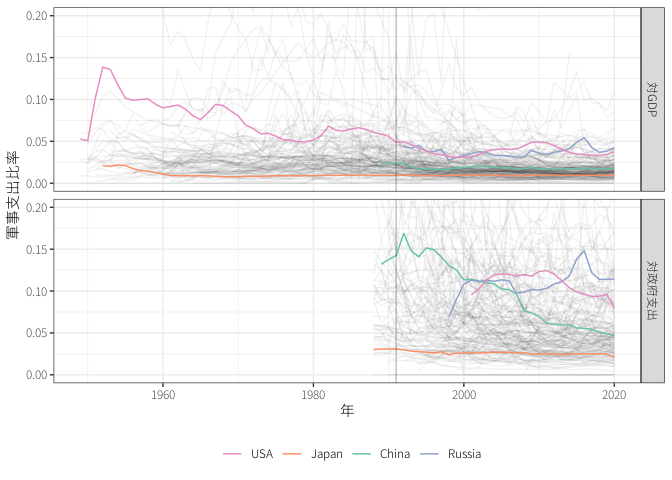
\includegraphics{democratic_peace_files/figure-pdf/unnamed-chunk-10-1.png}

}

\end{figure}

\textbf{安全保障外部性} (security
externalities):経済的相互依存から得られる利益は軍事力にも転換できる性質\citep{gowa1993}

\begin{itemize}
\tightlist
\item
  経済的相互依存の拡大\(\leadsto\)経済成長\(\leadsto\)軍事力も拡大\(\leadsto\)パワーシフト?
\end{itemize}

\hypertarget{ux7d4cux6e08ux5236ux88c1}{%
\subsection{経済制裁}\label{ux7d4cux6e08ux5236ux88c1}}

パワーとしての経済的相互依存\(\leadsto\)\textbf{経済制裁} (economic
sanction)

\begin{itemize}
\tightlist
\item
  経済制裁によって大きな打撃を与えることができるという点を貿易の武器化
  (weaponization of trade)
\item
  過度に経済的に相互依存しているので戦争をすることができないとして経済的相互確証破壊
  (mutulal assured economic destruction)
\end{itemize}

経済的相互依存の深化\(\leadsto\)経済制裁の威力を高める&経済制裁を行った側へのコストも高める\(\leadsto\)経済制裁が困難?

\begin{itemize}
\tightlist
\item
  自らは経済的相互依存から利益を得ていないが、相手は大きな利益を得ているときに効果
\item
  どのよう財を貿易しているのか、代替的な経済パートナーの有無などが重要?
\item
  グローバル化\(\leadsto\)経済的パートナーが増えると、ある国から経済制裁を受けても、他の国で代替が可能?
\end{itemize}

経済制裁による戦争の抑止効果

\begin{itemize}
\tightlist
\item
  戦争の機会費用を高める
\item
  継戦能力を損ない、勝利確率を低下
\item
  コストリーシグナルとして決意を伝達\citep{lektzian2007}
\end{itemize}

経済制裁が抑止効果を持っていないように見える理由

\begin{itemize}
\tightlist
\item
  一度、経済制裁を行うと、経済的相互依存の程度が下がってしまい、戦争の機会費用が低下

  \begin{itemize}
  \tightlist
  \item
    日本はアメリカからの石油禁輸で対米開戦を決意
  \end{itemize}
\item
  経済制裁を受けて戦争をやめる国はそもそも戦争を起こさない?
\item
  武力紛争が起こるほど対立している国とは経済的相互依存がもともと低い?
\end{itemize}

\(\leadsto\)経済制裁と軍事制裁の決定的な違いは実力による軍隊の排除や占領が可能か否か

\hypertarget{ux6771ux30a2ux30b8ux30a2ux306eux5e73ux548c}{%
\section{東アジアの平和?}\label{ux6771ux30a2ux30b8ux30a2ux306eux5e73ux548c}}

WW2以降、東アジアは例外的に平和を享受してきた。

\(\leadsto\)今後も平和を維持できるか?

\hypertarget{ux5e73ux548cux306eux52d5ux63faux30d1ux30efux30fcux30b7ux30d5ux30c8}{%
\subsection{平和の動揺:パワーシフト}\label{ux5e73ux548cux306eux52d5ux63faux30d1ux30efux30fcux30b7ux30d5ux30c8}}

WW2直後、中華人民共和国は国際社会に参加できず、また国力も乏しかった。

\begin{itemize}
\tightlist
\item
  改革開放以降の経済成長\(\leadsto\)軍事的台頭\(\leadsto\)秩序を変更する能力を持ち始める。
\item
  アメリカは中国の台頭を防止するための予防戦争を行う動機?
\end{itemize}

大国と急速に成長する台頭国の間で対立\(\leadsto\)戦争に至ることは歴史的に繰り返されてきた。

\begin{itemize}
\tightlist
\item
  ドイツの台頭はWW1の一因と考えられる。
\item
  アメリカの台頭、ソ連の挑戦、戦後のドイツ・日本の経済成長は戦争には繋がらず
\end{itemize}

\hypertarget{ux5e73ux548cux306eux8981ux56e0ux540cux76dfux3068ux7d4cux6e08}{%
\subsection{平和の要因:同盟と経済}\label{ux5e73ux548cux306eux8981ux56e0ux540cux76dfux3068ux7d4cux6e08}}

平和を維持するための要因のうち次のものは欠如

\begin{itemize}
\tightlist
\item
  集団安全保障:アメリカと中国はP5なので安保理は機能できない。
\item
  地域的な安全保障機構:存在せず
\item
  民主的平和:権威主義国の中国や北朝鮮
\end{itemize}

\(\leadsto\)消去法的に今後の東アジアの平和を維持する要因は同盟と経済的相互依存?

\begin{itemize}
\tightlist
\item
  同盟はアメリカの能力とコミットメント(特に核兵器による拡大抑止)次第
\item
  経済的相互依存は商業的平和と経済安全保障のジレンマ
\end{itemize}

\hypertarget{ux3044ux304fux3064ux304bux306eux30b7ux30caux30eaux30aa}{%
\subsection{いくつかのシナリオ}\label{ux3044ux304fux3064ux304bux306eux30b7ux30caux30eaux30aa}}

悲観的シナリオ:アメリカと中国の利害は衝突し、影響力拡大のために衝突

\begin{itemize}
\tightlist
\item
  人権や民主主義、経済体制に関する価値観の違い
\item
  日本や韓国、台湾、フィリピンにおけるアメリカの軍事的プレゼンス、コミットメント\(\leadsto\)譲歩できず
\item
  中国は台湾問題で譲歩できず
\end{itemize}

\(\leadsto\)中国との経済交流を制限して成長を抑制&軍事力を拡大して抑止する\textbf{封じ込め}
(containment)

楽観的シナリオ:中国は既存の国際秩序から利益&責任ある大国として行動

\begin{itemize}
\tightlist
\item
  中国は自由な国際経済秩序によって経済成長を実現、貿易や投資パートナーはアメリカやその同盟国
\item
  安保理常任理事国として受け入れ、IMFや世銀でも投票権を拡大
\item
  経済成長は人権や民主主義の価値観を受け入れやすくする?
\end{itemize}

\(\leadsto\)中国を様々な国際制度に参加させ、現状の利益を拡大させる\textbf{関与}
(engagement) 政策

アメリカは軍事的な封じ込めと経済的関与\(\leadsto\)経済的にも封じ込め?

\begin{itemize}
\tightlist
\item
  中国の経済活動の制限(特に知的財産)&アメリカにおける雇用の喪失\(\leadsto\)トランプ政権が\textbf{貿易戦争}
  (trade war)
\item
  バイデン政権においても、抜本的な政策転換が起こっているとは言えない。
\item
  孤立主義的な共和党大統領が登場すると同盟コミットメントも疑わしくなる。
\end{itemize}

中国については分からないことが多いが、1つの要因は経済成長と人口成長の鈍化?

\begin{itemize}
\tightlist
\item
  中国の台頭が緩やかになり、現状の維持に満足する軟着陸コース
\item
  将来の衰退を恐れて、有利な時点での予防的挑戦
\end{itemize}


  \bibliography{references.bib}


\end{document}
